%!TEX root = main.tex
\section{Towards Intelligent Visual Search}\label{sec:vague}
\subsection{The Challenge of Usability-Expressivity Tradeoff}
\par The challenge for supporting vague and complex querying stems from the inevitable design trade-off between query expressivity and interface usability in interactive data exploration systems~\cite{Jagadish2007,Morton2014}. This tradeoff is observed not only in visual data exploration systems, but also true for general ad-hoc data querying. While querying language such as SQL are highly expressive, formulating SQL queries that maps user's high-level intentions to specific query statements is challenging~\cite{Jagadish2007,Khoussainova2010}. As a result, query construction interfaces have been developed to address this issue by enabling direct manipulation of queries through graphical representations~\cite{Abouzied2012}, gestural interaction~\cite{Nandi2013}, and tabular inputs~\cite{Zloof1975,Embley1989}. For example, form-based query builders often consist of highly-usable interfaces that ask users for a specific set of information mapped onto a pre-defined query. However, form-based query builders are often based on query templates with limited expressiveness in their semantic and conceptual coverage, which makes it difficult for expert users to express complex queries. The extensibility of these systems also comes with the high engineering cost, as well as potentially overloading the users with too many potential options to chose from. There is a need for tools that is enables users to formulate rich and complex queries, yet highly usable even for novices.  
%Most systems design exhibits a trade-off between how expressive can the query be and how usable the interface is. 

% \begin{itemize}
% \item Inferring user intent in querying and context is important (both in terms of user input and what is recommended)
% \item tools can not assume user has querying intention. exploration without intention, user don’t know what they are searching for --> Recommendation.
% \item The important thing here is identifying what should be done by the system v.s. requested from user. Inappropriate choice of these will result in lack of expressibility and user feeling lack of control of analysis, limiting exploration.
% \item 
% \end{itemize}
\subsection{Ongoing research and opportunities}
\par Given the tradeoff between expressivity and usability, we can not assume a one-size-fit-all PVQS that could fit the needs for users of different expertise levels and workloads. In this section, we discuss a growing class of \textit{intelligent visual querying system} (IVQS) that works around this problem by taking into account queries of varying degrees of input specificity. There are many open research questions in accelerating the discovery process of answering an imprecise, fuzzy, and complex queries, including : How can we develop better ways to resolve ambiguity by infering the information needs and intent of an analyst? What is the appropriate level of feedback and interactions in IVQSs? How can we develop interpretable visual metaphors that could serve to explain how the query was interpreted and why specific query results are returned to a lay user?
 We describe three different system challenges in interpreting non-precise queries. Since most visual query systems operates on top of a querying language, we use the linguistical classification scheme to provide an analogy for where the ambiguous aspects of queries may arise during visual data exploration, noting that the use of this analogy by no means limits our analysis to only natural language interfaces.

\begin{figure}[h!]
\centering
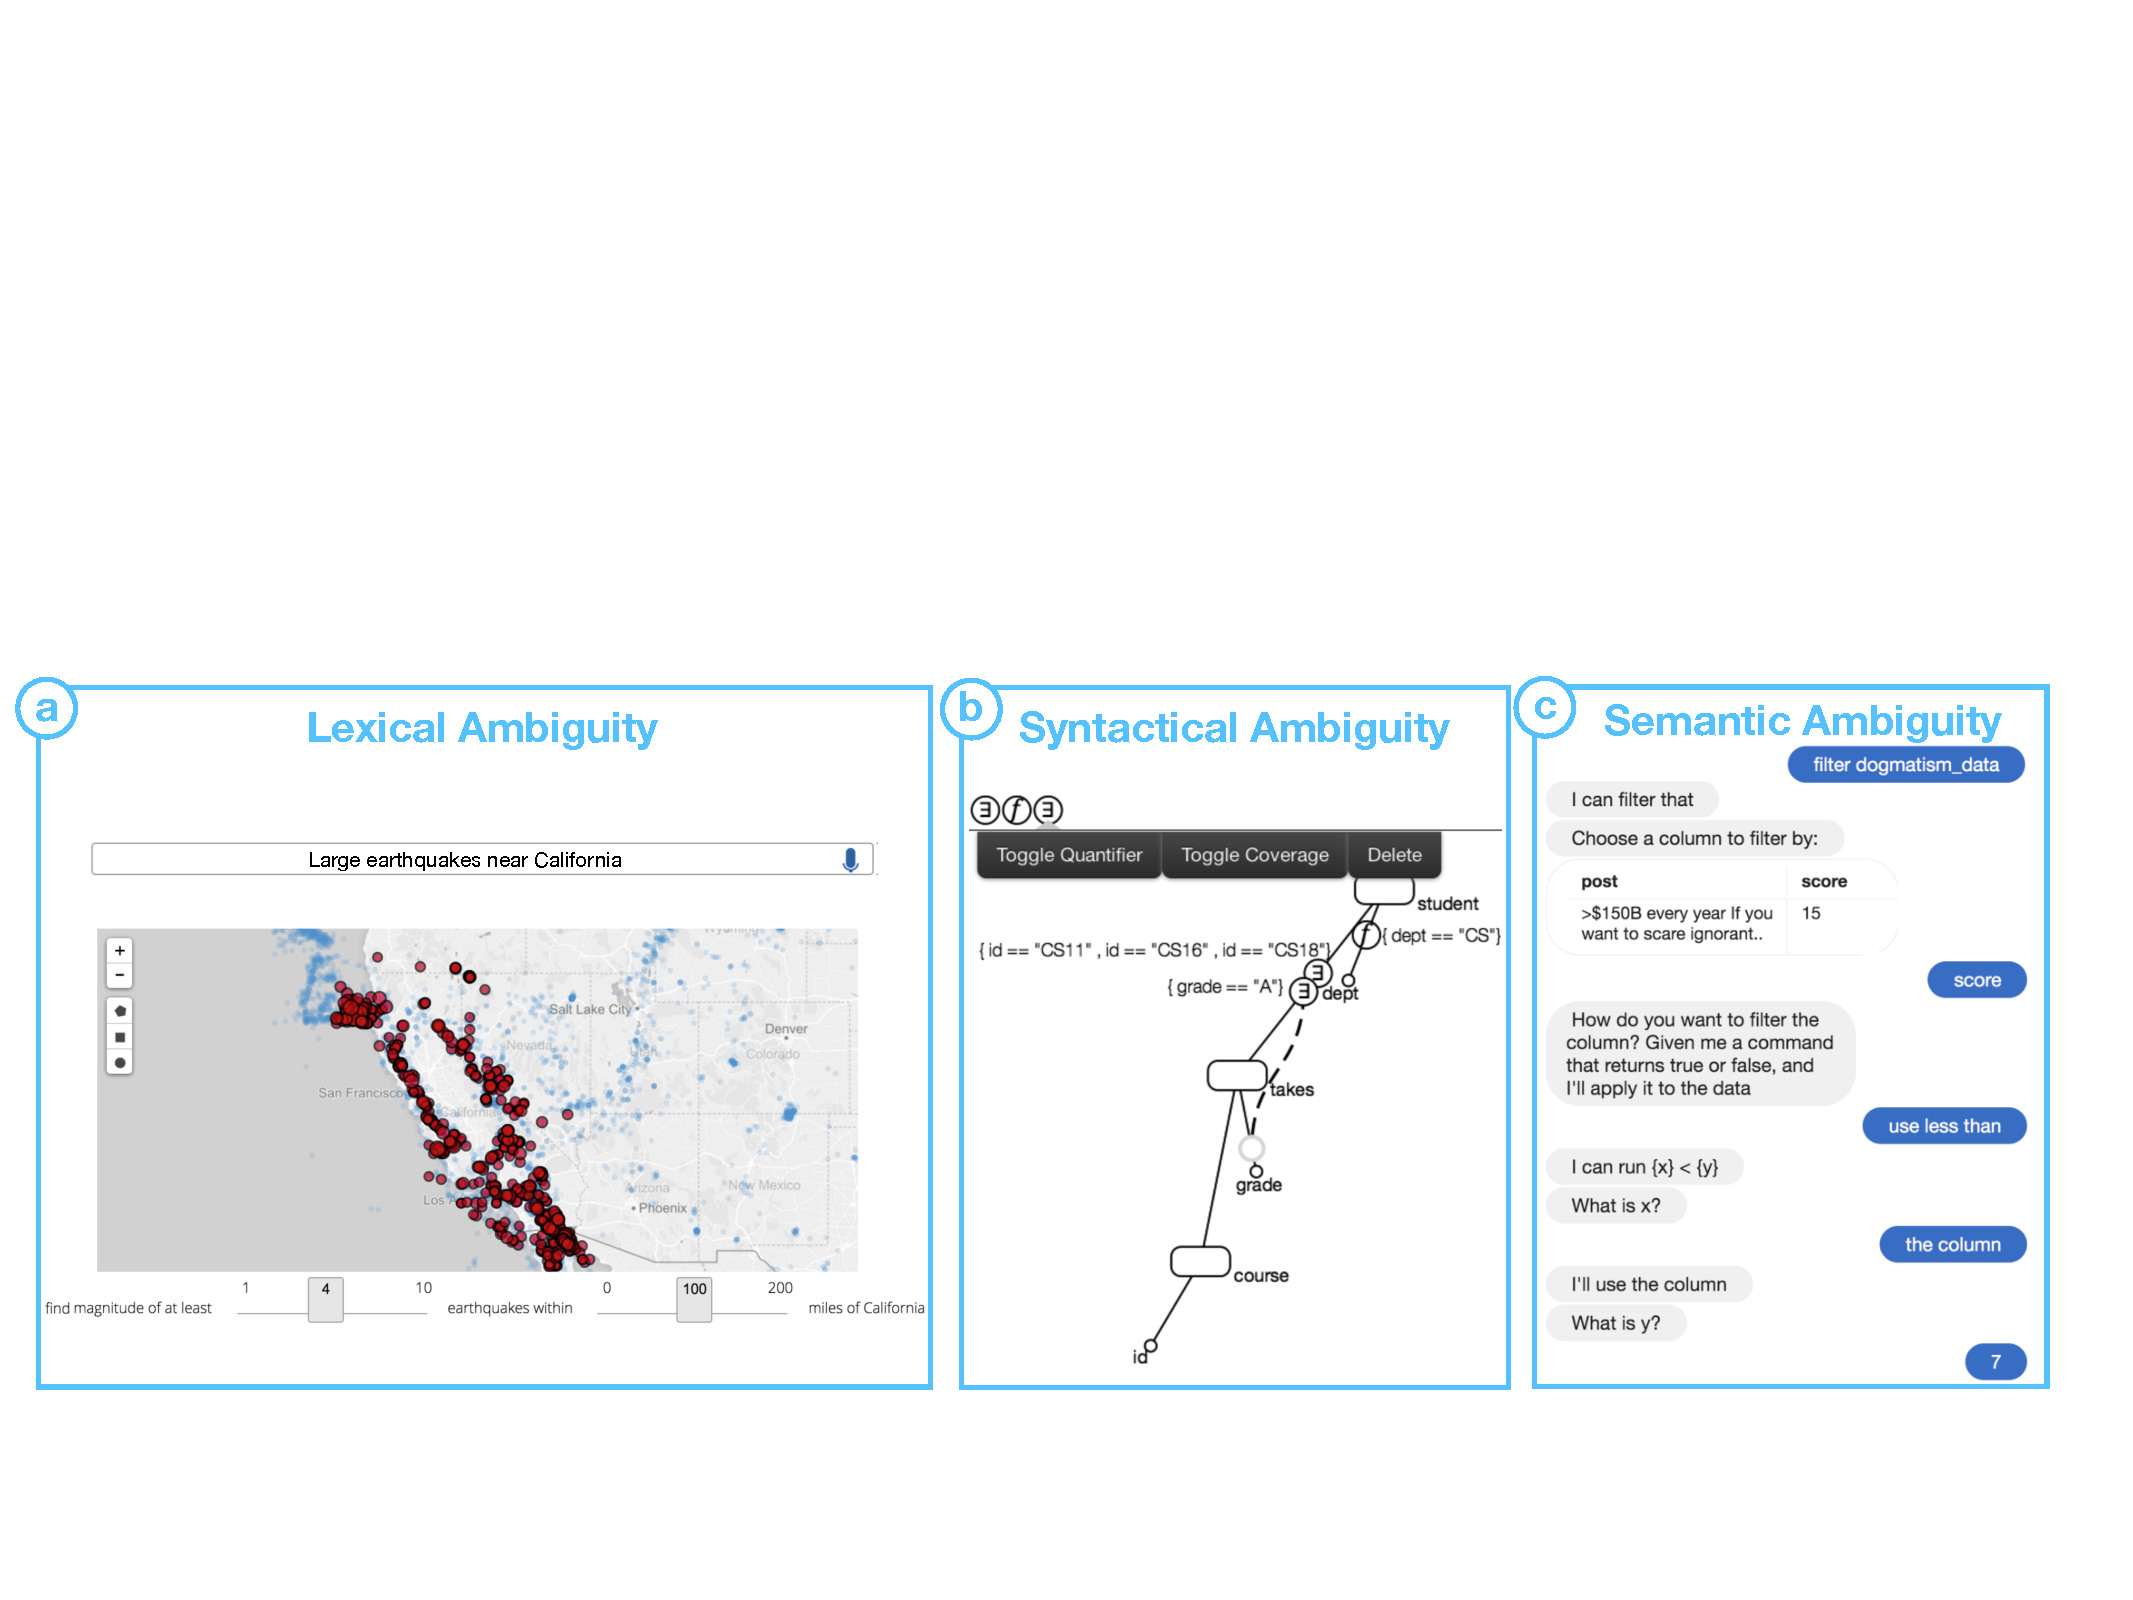
\includegraphics[width=\textwidth]{figures/ambiguity.pdf}
\caption{Examples of IVQSs: a) Eviza~\cite{Setlur2016} uses ambiguity widgets to enable users to clarify vaguely-defined terms in their input query to resolve lexical ambiguity; b) DataPlay~\cite{Abouzied2012} allow users to toggle between `for all' and `at least one' quantifier to control for syntactical ambiguity; c) Iris~\cite{Fast2018} accepts a vague high-level task description and gather the additional information required through follow-up questions in a nested conversation.}
\label{fig:ambiguity}
\end{figure}
\stitle{Lexical Ambiguity}: Lexical ambiguity involves the use of vague descriptors in the input queries. Resolving these lexical ambiguities has been a subject of research in natural language interfaces (NLIs) for visualization specification, such as DataTone~\cite{Gao2015} and Eviza~\cite{Setlur2016}. These NLIs detects ambiguous quantifiers in the input query (e.g. ``Large earthquakes near California''), and then displays ambiguity widgets in the form of a widget to allow users to specify the definition of `large' in terms of magnitude and the number of miles radius for defining `near', as shown in Figure~\ref{fig:ambiguity}a. These ambiguity widgets not only serve as a way to provide feedback to the system for lexically vague queries, but also is a way for displaying interpretable explanations of how the system is interpreting the input queries. If we consider IVQSs as a layer on top of PVQS (that performs functionalities such as shape-matching, filtering), an IVQS resolves lexical ambiguity by determining the appropriate \textit{parameters} to the PVQS to achieve the user's desired querying effects.
% For example,  NaLIR (explanation through query tree, and display multiple interpretations), Eviza (ambiguity widgets), both Eviza/Iris/Ava (follow on clarification utterances). 
\dor{Describe ShapeSearch here}
\stitle{Syntactic Ambiguity}: Syntactic ambiguity is related to the vagueness in specifying how the query should be structured or ordered. For example, DataPlay introduced the idea of syntax non-locality in SQL, in which switching from an existential (at least one) to a universal (for all) quantifier requires major structural changes to the underlying SQL query~\cite{Abouzied2012}. As shown in Figure~\ref{fig:ambiguity}b, DataPlay consist of a visual interface that allowed users to directly manipulate the structure of the query tree in tweaking the query to its desired specification. IVQSs resolve syntactic ambiguities either by mapping portions of the vague queries into to \textit{a series of multi-step workflows} to be executed in the PVQS and allow users to tweak the query representation directly. The query modification is done in a declarative manner in that the underlying mechanism in which the visualized workflow gets translated to the querying language is largely hidden from the end-user. 
\stitle{Semantic Ambiguity}: Semantic ambiguity arises when the user does not specify their intent completely or explicitly, which is often the case in the earlier stages of the visual data exploration. NLIs for visual data exploration such as Evizeon~\cite{Hoque2017} makes use of anaphoric references to fill in incomplete follow-on queries. For example, when a user says `Show me average price by neighborhood', then `by home type', the system interprets the anaphoric reference as continuing the context of the original utterance related to average price on the y-axis. Semantic ambiguity can often be composed of one or more lexical and syntactical ambiguity. For example, in Iris~\cite{Fast2018}, a user can specify a vague, high-level query such as `Create a classifier', then Iris makes use of nested conversations to inquire about what type of classifier to chose and what features to use in the model to fill in the details of the structure and parameters required. A semantically vague query may or may not be expressible through a single PVQS, since the operations involved in the query may not be covered by the limited workflow combinations in the PVQS. 
% Another form of syntactic ambiguity is how  through followup query tweaking 
% nested queries and anaphoric references~\cite{Hoque2017}. Show me relationship between price and -----, then "Break down by -----".
% user intention, composition , Accounting for user interaction, mental models. More global objective taking into account user with the goal of dataset understanding rather than task completion. Need for a unified framework of inference to take all of these into account (e.g. natural language, etc)


%ble to functionalities required to ---- full intent. 

% \stitle{Vague and Ambiguous querying}
 

% \stitle{Recommendation}
% Multimodal visual interfaces, inferring intent from interaction data
% As illustrated in Fig.\ref{system}, these can range from cold-start (no supervision) to input examples, input relations to complete specification.
% \stitle{Complex composition}
% nesting (Ava and Iris)
% In PVQS, the actions are independent of when you do it, when you do them, because they could all be considered as independent series of operations. 

% \par natural language interfaces 
% - joining the flow 
% is a need for an vague or ambiguous specification and global mechanism for ---- nesting ---formulated complex combination. 